\documentclass{report}
\usepackage{pgf,tikz,pgfplots}
\pgfplotsset{compat=1.15}
\usepackage{mathrsfs}
\usetikzlibrary{arrows}
\usepackage{float}
\usepackage{cancel}
\usepackage{enumerate}
\usepackage{amsmath}

\title{Solutions for Calculus Vol 1: One variable calculus, with an introduction to Linear Algebra (2nd Edition) by Tom M. Apostol}
\author{Michael Rocke}

\begin{document}
\maketitle

\tableofcontents

\section{Introduction}

\subsection{1.4 Exercises}

\subsubsection{1}

\begin{figure}[H]

		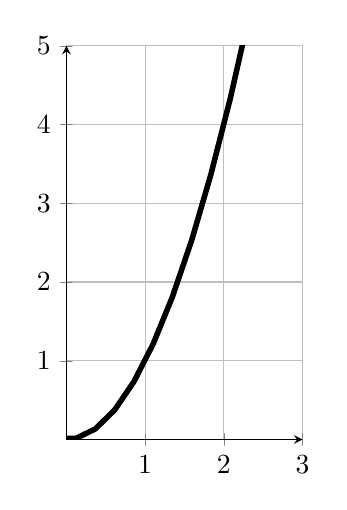
\begin{tikzpicture}[line cap=round,line join=round,>=triangle 45,x=1cm,y=1cm]
		\begin{axis}[
		x=1cm,y=1cm,
		axis lines=middle,
		ymajorgrids=true,
		xmajorgrids=true,
		xmin=0,
		xmax=3,
		ymin=0,
		ymax=5,
		xtick={-12,-11,...,4},
		ytick={-9,-8,...,9},]
		\clip(-12.92,-9.52) rectangle (4.92,9.52);
		\draw [samples=50,rotate around={0:(0,0)},xshift=0cm,yshift=0cm,line width=2pt,domain=-6:6)] plot (\x,{(\x)^2/2/0.5});
		\begin{scriptsize}
		\draw[color=black] (-1.7,1.03) node {$y = x^2$};
		\end{scriptsize}
		\end{axis}
		\end{tikzpicture}
		
		Figure 1.3: $y=x^2$
\end{figure}

a) Modify the region in Figure 1.3 by assuming that the ordinate at each $x$ is $2x^2$ instead of $x^2$. 

Draw the new figure. 

\begin{figure} [H]
	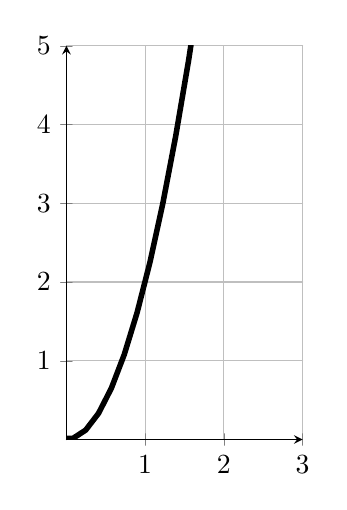
\begin{tikzpicture}[line cap=round,line join=round,>=triangle 45,x=1cm,y=1cm]
	\begin{axis}[
	x=1cm,y=1cm,
	axis lines=middle,
	ymajorgrids=true,
	xmajorgrids=true,
	xmin=0,
	xmax=3,
	ymin=0,
	ymax=5,
	xtick={-12,-11,...,4},
	ytick={-9,-8,...,9},]
	\clip(-12.92,-9.52) rectangle (4.92,9.52);
	\draw [samples=50,rotate around={0:(0,0)},xshift=0cm,yshift=0cm,line width=2pt,domain=-4:4)] plot (\x,{(\x)^2/2/0.25});
	\begin{scriptsize}
	\draw[color=black] (-1.12,0.53) node {$y = 2x^2$};
	\end{scriptsize}
	\end{axis}
	\end{tikzpicture}
	
	$y = 2x^2$
\end{figure}

Check through the principal steps in the forgoing section and find what effect this has on the calculation of the area. Do the same if the ordfinate at each $x$

b) $3x^2$

\begin{figure}[H]

		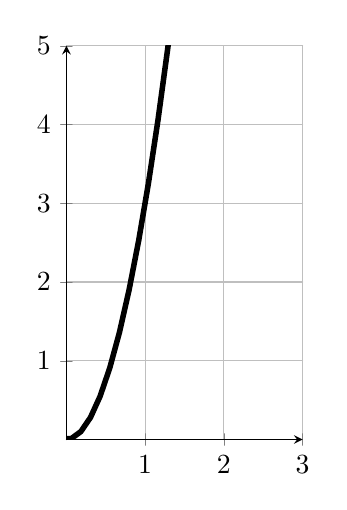
\begin{tikzpicture}[line cap=round,line join=round,>=triangle 45,x=1cm,y=1cm]
		\begin{axis}[
		x=1cm,y=1cm,
		axis lines=middle,
		ymajorgrids=true,
		xmajorgrids=true,
		xmin=0,
		xmax=3,
		ymin=0,
		ymax=5,
		xtick={-12,-11,...,4},
		ytick={-9,-8,...,9},]
		\clip(-12.92,-9.52) rectangle (4.92,9.52);
		\draw [samples=50,rotate around={0:(0,0)},xshift=0cm,yshift=0cm,line width=2pt,domain=-3:3)] plot (\x,{(\x)^2/2/0.16666666666666666});
		\begin{scriptsize}
		\draw[color=black] (-0.96,0.37) node {$y = 3x^2$};
		\end{scriptsize}
		\end{axis}
		\end{tikzpicture}
		
		$y = 3x^2$
\end{figure}

c) $\frac{1}{4}x^2$

\begin{figure}[H]
	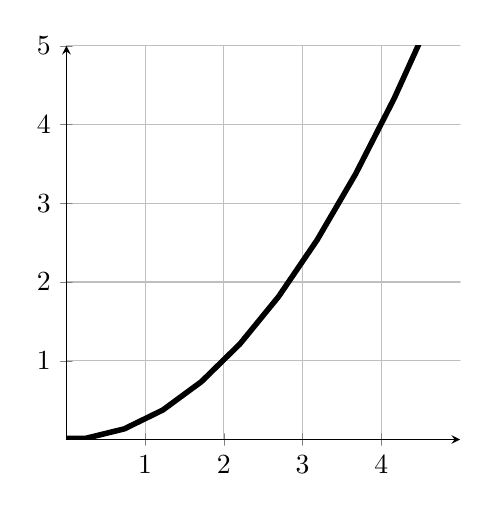
\begin{tikzpicture}[line cap=round,line join=round,>=triangle 45,x=1cm,y=1cm]
	\begin{axis}[
	x=1cm,y=1cm,
	axis lines=middle,
	ymajorgrids=true,
	xmajorgrids=true,
	xmin=0,
	xmax=5,
	ymin=0,
	ymax=5,
	xtick={-12,-11,...,4},
	ytick={-9,-8,...,9},]
	\clip(-12.92,-9.52) rectangle (4.92,9.52);
	\draw [samples=50,rotate around={0:(0,0)},xshift=0cm,yshift=0cm,line width=2pt,domain=-12:12)] plot (\x,{(\x)^2/2/2});
	\begin{scriptsize}
	\draw[color=black] (-4.38,4.03) node {$y = x^2 / 4$};
	\end{scriptsize}
	\end{axis}
	\end{tikzpicture}
	
	$y = \frac{1}{4} x^2$
\end{figure}

d) $2x^2 + 1$

e) $ax^2 + c$

\subsubsection{2}

Modify the region in Figure 1.3 by assuming that the ordinate at each $x$ is $x^3$ instead of $x^2$.

Draw the new figure.

a) Use a construction similar to that illustrated in Figure 1.5 and show that the outer and inner sums $S_n$ and $s_n$ are given by

\[
S_n = \frac{b^4}{n^4} (1^3 + 2^3 + ... + n^3), \; s_n = \frac{b^4}{n^4}[1^3 + 2^3 + ... + (n - 1)^3]
\]


b)

\section{The concepts of integral calculus}

\subsection{1.5 Exercises}

\subsubsection{1}

Let $f(x) = x + 1$ for al real x. Compute the following

$f(2) = 3$

$f(-2) = -1$

$-f(2) = -3$

$f(\frac{1}{2})= \frac{3}{2}$

$1/f(2) = \frac{1}{3}$

$f(a + b) = a + b + 1$

$f(a) + f(b) = a + b + 2$

$f(a)f(b) = (a+1)(b+1) = ab + a + b + 1$

\subsubsection{2}

Let $f(x) = 1 + x$ and let $g(x) = 1 - x$ for all real x. Compute the following:

$f(2) + g(2) = 3 + (-1) = 2$

$f(2) - g(2) = 3 - (-1) = 4$

$f(2)g(2) = -3$

$f(2)/g(2) = -3$

$f[g(2)] = f(-1) = 0$

$g[f(2)] = g[3] = -2$

$f(a) + g(-a) = 1 + a + (1 - (-a)) = 2 + 2a$

$f(t)g(-t) = (1 + t)(1 - (-t)) = 1 + 2t + t^2$

\subsubsection{3}

Let $\psi(x) = |x - 3| + |x -1|$ for all real x. Compute the following:

$\psi(0) = |0 - 3| + |0 - 1| = 3 + 1 = 4$

$\psi(1) = |1 - 3| + |1 - 1| = 2$

$\psi(2) = |2 - 3| + |2 - 1| = 1 + 1 = 2$

$\psi(3) = |3 - 3| + |3 - 1| = 2$

$\psi(-1) = |-1 - 3| + |-1 - 1| = 6$

$\psi(-2) = |-2 - 3| + |-2 - 1| = 5 + 3 = 8$

Find all $t$ for which $\psi(t + 2) = \psi(t)$
$\psi(t) = |t - 3| + |t - 1|$
$\psi(t+2) = |t + 2 - 3| + |t + 2 - 1| = |t - 1| + |t + 1| $

Given $|t - 3| + \cancel{|t - 1|} = \cancel{|t - 1|} + |t + 1|$ 

thus $|t - 3| = |t + 1|$

Only value that will satisfy is when $t = 1$

\subsubsection{4}

Let $f(x) = x^2$ for all real x. Verify each of the following formulas. In each case describe the set of real x, y, t, etc., for which the given formula is valid

\begin{enumerate}[(a)]
	\item $f(-x) = f(x)$, So $	f(-x) =(-x)\cdot(-x) = (x) \cdot (x) = f(x)$ for all x
	\item $f(y) - f(x) = (y-x)(y+x)$, So $(y-x)(y+x) = y^2 - x^2 = f(y) - f(x)$ for all x and y
	\item $f(x+h) - f(x) = 2xh + h^2$, So, $f(x+h) - f(x) = (x+h)^2 - x^2 = \cancel{x^2} + 2xh + h^2 - \cancel{x^2}$ for all x and h
	\item $f(2y) = 4f(y)$, So $f(2y) = (2y)^2 = 4y^2 = 4f(y)$ for all y
	\item $f(t^2) = f(t)^2$, So $f(t^2) = (t^2)^2 = f(t)^2$ for all t
	\item $\sqrt{f(a)} = |a|$, So $\sqrt{f(a)} = \sqrt{a^2}$ which when taking the positive root, is $|a|$ for all a
\end{enumerate}


\end{document}